%
% oc.tex -- einfache Bespiele
%
% (c) 2024 Prof Dr Andreas Müller
%
\begin{figure}
\centering
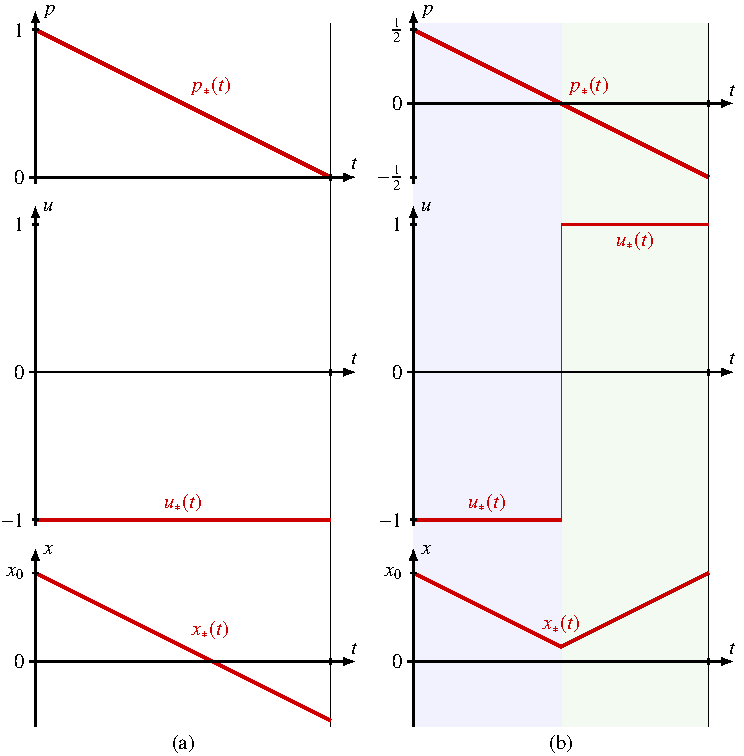
\includegraphics{chapters/080-hamiltonjacobi/images/oc.pdf}
\caption{Beispiele für einfache optimale Steuerungsprobleme.
In allen Beispielen wird immer von oben nach unten erst die Funktion
$p_*(t)$ aus den Hamilton-Differentialgleichungen bestimmt.
Mit dem Minimum-Prinzip von Pontryagin kann dann $u_*(t)$ bestimmt
werden.
Aus $u_*(t)$ ergibt sich schliesslich $x_*(t)$ mit der
Systemdifferentialgleichung
In Beispiel~\ref{buch:hamiltonjacobi:oc:bsp:simple}, (a), ist die
optimale Wahl von $u_*(t)=-1$, im
Beispiel~\ref{buch:hamiltonjacobi:oc:bsp:switch}, (b), schaltet die
optimale Steuerfunktion beim Vorzeichenwechsel von $p_*(t)$ vom
Wert $-1$ zum Wert $1$ um.
\label{buch:hamiltonjacobi:oc:fig:oc}}
\end{figure}
